\section{Testes A/B Computacionais}

\begin{frame}{Comparando Dois Grupos Independentes}
    \begin{block}{Duas Abordagens Didáticas}
        \begin{enumerate}
            \item \textbf{Sobreposição de ICs Individuais:} Calcular o IC para cada grupo separadamente e checar se eles se sobrepõem. (Abordagem conservadora).
            \item \textbf{IC da Diferença das Médias (Padrão):} Estimar diretamente a distribuição bootstrap de $\bar{X}_1 - \bar{X}_2$. Se o intervalo correspondente contiver o valor zero, dizemos que não há diferença significativa entre as médias.
        \end{enumerate}
    \end{block}
\end{frame}

\begin{frame}{Exemplo Matemático: Diferença de Médias via Bootstrap}
    \begin{block}{Problema}
        Grupos: $X_A = \{10, 15, 20\} \rightarrow \bar{X}_A = 15.0$ e $X_B = \{12, 18, 24\} \rightarrow \bar{X}_B = 18.0$.
        Diferença observada: $+3.0$. Vamos reamostrar com reposição:
    \end{block}
    \begin{block}{Simulações de Reamostragem}
        \begin{itemize}
            \item \textbf{Passo 1:} Reamostras $B^*_1 = \{18, 24, 24\}$ (méd. $22.0$) e $A^*_1 = \{15, 15, 20\}$ (méd. $16.67$). Diferença: $22.0 - 16.67 = 5.33$.
            \item \textbf{Passo 2:} Reamostras $B^*_2 = \{12, 12, 18\}$ (méd. $14.0$) e $A^*_2 = \{10, 20, 20\}$ (méd. $16.67$). Diferença: $14.0 - 16.67 = -2.67$.
        \end{itemize}
        Repetindo 5000 vezes, analisamos se a diferença é significativamente maior que zero.
    \end{block}
\end{frame}

\begin{frame}[fragile]{Demonstração em Python: Teste A/B Simples}
    \begin{lstlisting}[language=Python]
import numpy as np

# Grupos originais
grupo_A = np.array([10, 15, 20])
grupo_B = np.array([12, 18, 24])

# Simulando a diferenca das medias
np.random.seed(42)
diferencas_bs = []

for _ in range(5000):
    resample_A = np.random.choice(grupo_A, size=len(grupo_A), replace=True)
    resample_B = np.random.choice(grupo_B, size=len(grupo_B), replace=True)
    diferencas_bs.append(resample_B.mean() - resample_A.mean())

# Intervalo de Confianca de 95% para a diferenca
ic_diferenca = np.percentile(diferencas_bs, [2.5, 97.5])
print(f"IC da diferenca (95%): [{ic_diferenca[0]:.2f}, {ic_diferenca[1]:.2f}]")
# Saida: IC da diferenca (95%): [-3.67, 9.67]. Contem zero, nao e significativa!
    \end{lstlisting}
\end{frame}


\begin{frame}[fragile]{Caso de Estudo 1: Saúde Pública}
    \begin{block}{Peso de Bebês e Tabagismo Materno}
        \begin{itemize}
            \item \textbf{Dados:} Amostra de recém-nascidos (\texttt{baby.csv}).
            \item \textbf{Grupo Controle:} Mães não fumantes.
            \item \textbf{Grupo Tratamento:} Mães fumantes.
        \end{itemize}
    \end{block}
    
    \begin{lstlisting}[language=Python]
# Codigo para calcular diferenca de medias via bootstrap
def bootstrap_diff(df1, df2, column, n=5000):
    data1 = df1[column].to_numpy()
    data2 = df2[column].to_numpy()
    diff_values = np.zeros(n)
    for i in range(n):
        s1 = np.random.choice(data1, size=len(df1), replace=True)
        s2 = np.random.choice(data2, size=len(df2), replace=True)
        diff_values[i] = s1.mean() - s2.mean()
    return diff_values
    \end{lstlisting}
\end{frame}

\begin{frame}[fragile]{Código Completo: Carga, Preparação e Bootstrap}
    \begin{lstlisting}[language=Python]
import pandas as pd
import numpy as np

# 1. Carregar dados da URL
url = 'https://media.githubusercontent.com/media/icd-ufmg/material/master/aulas/10-AB/baby.csv'
df = pd.read_csv(url)

# 2. Conversao de unidades (oncas para kg)
df['Birth Weight'] = 0.0283495 * df['Birth Weight']

# 3. Separar em grupos: Controle vs Tratamento
smokers = df[df['Maternal Smoker'] == True]
no_smokers = df[df['Maternal Smoker'] == False]

# 4. Rodar o bootstrap para a diferenca das medias
np.random.seed(42)
diferencas = bootstrap_diff(smokers, no_smokers, 'Birth Weight', n=5000)

# 5. Calcular o IC de 95 por cento para a diferenca
ic_95 = np.percentile(diferencas, [2.5, 97.5])
print(f"IC 95%: [{ic_95[0]:.3f} kg, {ic_95[1]:.3f} kg]")
    \end{lstlisting}
\end{frame}

\begin{frame}{Resultados: Peso de Bebês}
    \begin{itemize}
        \item \textbf{Média não fumantes:} $3.489\text{ kg}$
        \item \textbf{Média fumantes:} $3.227\text{ kg}$
        \item \textbf{Diferença observada:} $-0.263\text{ kg}$
        \item \textbf{IC de 95\% para a diferença (Bootstrap):} $[-0.323, -0.202]\text{ kg}$
    \end{itemize}
    
    \begin{alertblock}{Conclusão Estatística}
        Como o intervalo $[-0.323, -0.202]\text{ kg}$ \textbf{não inclui o valor zero}, rejeitamos a hipótese de igualdade entre as médias. Há diferença estatística significativa.
    \end{alertblock}
\end{frame}

\begin{frame}{Visualização: Distribuições de Médias Bootstrap}
    \centering
    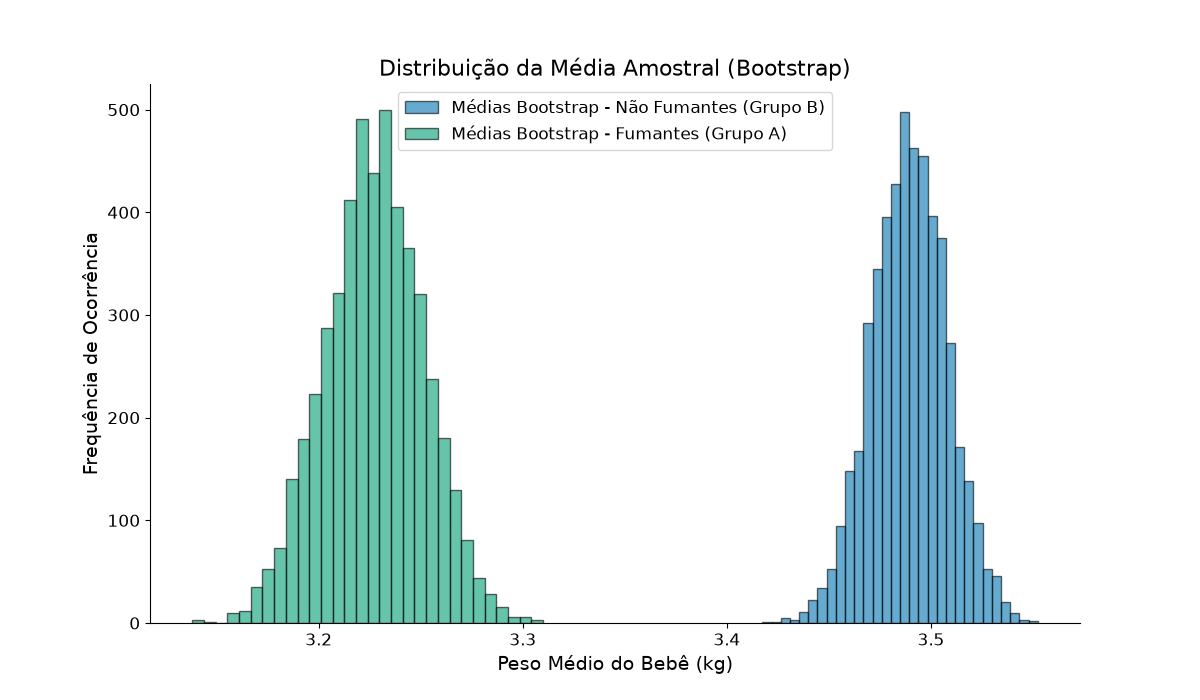
\includegraphics[width=0.85\textwidth]{02_medias_bootstrap.png}
\end{frame}

\begin{frame}{Explicação: Distribuições das Médias Bootstrap}
    \begin{block}{Interpretação das Médias Individuais}
        \begin{itemize}
            \item \textbf{Mães Não Fumantes (azul):} A distribuição das médias amostrais $\bar{X}$ (média amostral) está centrada em $3.49\text{ kg}$, variando no $IC$ (Intervalo de Confiança) de $[3.45, 3.52]\text{ kg}$.
            \item \textbf{Mães Fumantes (laranja):} A distribuição está centrada em $3.23\text{ kg}$, variando no $IC$ (Intervalo de Confiança) de $[3.18, 3.27]\text{ kg}$.
            \item \textbf{Ausência de Sobreposição:} Como os $IC$ (Intervalos de Confiança) dos dois grupos não se sobrepõem, há um indício inicial muito forte de que o peso médio populacional é diferente entre os grupos.
        \end{itemize}
    \end{block}
\end{frame}

\begin{frame}{Visualização: Diferença de Médias e ECDF}
    \centering
    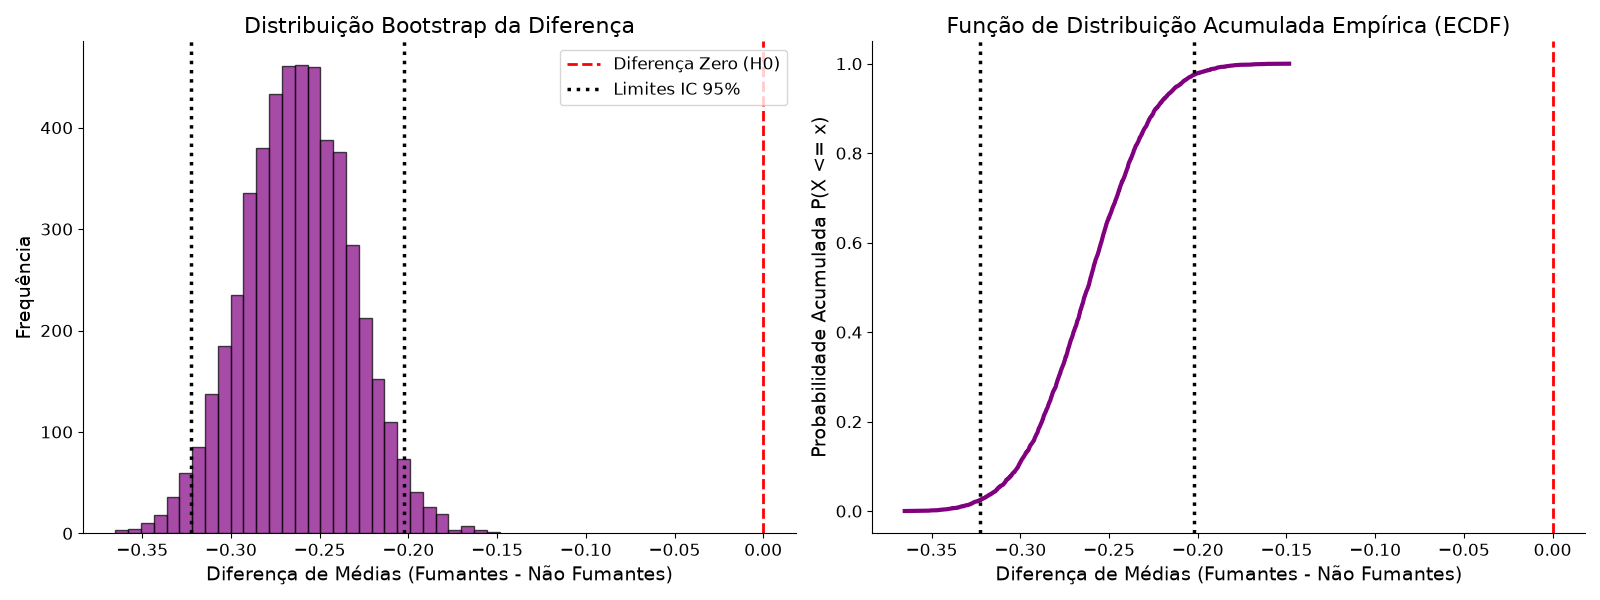
\includegraphics[width=0.9\textwidth]{03_diferenca_ecdf.png}
\end{frame}

\begin{frame}{Explicação: Efeito da Diferença e ECDF}
    \begin{block}{Análise da Diferença e da ECDF}
        \begin{itemize}
            \item \textbf{Distribuição da Diferença (Esquerda):} Mostra a distribuição de todas as $5.000$ diferenças simuladas $\bar{d}^* = \bar{X}^*_{\text{Fumantes}} - \bar{X}^*_{\text{Não Fumantes}}$. O $IC$ (Intervalo de Confiança) de 95\% da diferença é $[-0.323, -0.202]\text{ kg}$ (totalmente abaixo de zero).
            \item \textbf{Curva ECDF (Direita):} A $ECDF$ (Função de Distribuição Acumulada Empírica) chega ao topo ($1.0$ ou 100\% de probabilidade acumulada) bem antes do ponto zero no eixo horizontal.
            \item \textbf{Conclusão:} A probabilidade de a diferença ser maior ou igual a zero é nula ($P(\bar{d}^* \ge 0) = 0$), comprovando o efeito negativo do fumo.
        \end{itemize}
    \end{block}
\end{frame}

\begin{frame}{Caso de Estudo 2: UX e E-commerce}
    \begin{block}{Impacto de Checkout Expresso no Ticket Médio}
        \begin{itemize}
            \item \textbf{Layout A (Controle):} Checkout em múltiplos passos (250 vendas). Média: R\$44.75.
            \item \textbf{Layout B (Tratamento):} Novo Checkout Expresso (200 vendas). Média: R\$47.29.
        \end{itemize}
    \end{block}
    
    \begin{block}{Simulação Bootstrap do Ticket Médio}
        \begin{itemize}
            \item Diferença de médias observada (B - A): $+\text{R\$} 2.53$
            \item IC de 95\% da diferença: $[\text{R\$} 0.18, \text{R\$} 4.90]$
            \item \textbf{Conclusão:} Como o limite inferior de R\$0.18 está acima de zero, podemos afirmar que o novo layout gerou aumento de receita.
        \end{itemize}
    \end{block}
\end{frame}

\begin{frame}{Visualização: Dispersão do Ticket Médio}
    \centering
    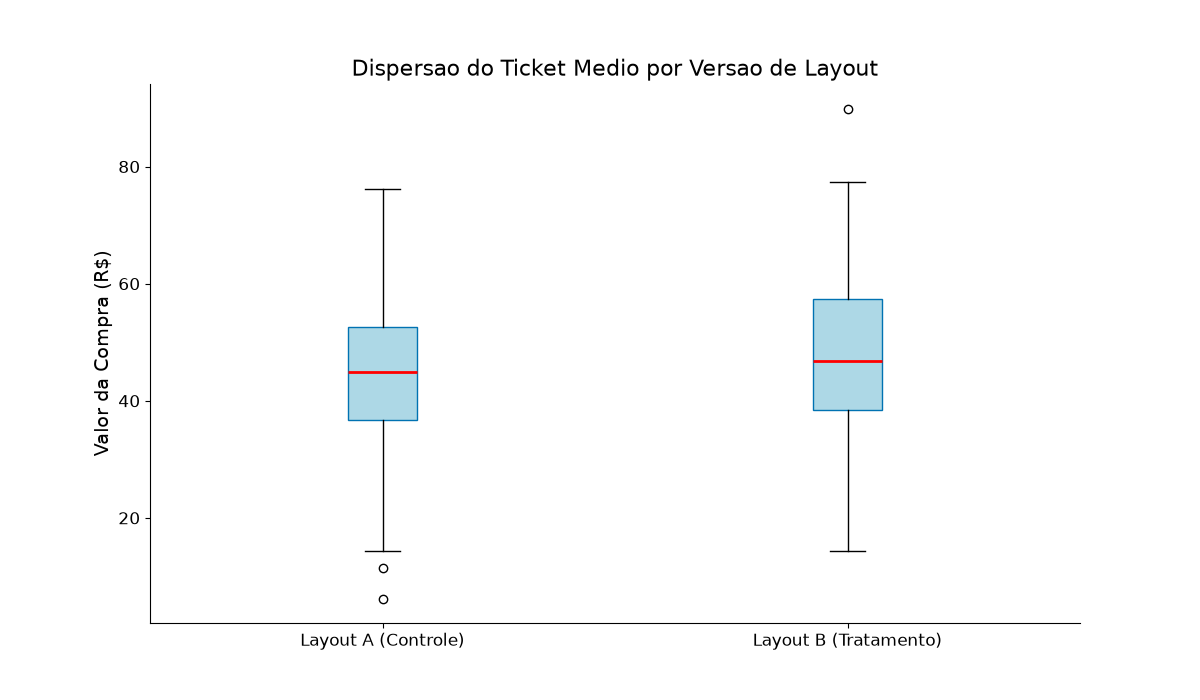
\includegraphics[width=0.85\textwidth]{05_boxplot_ecommerce.png}
\end{frame}

\begin{frame}{Explicação: Boxplot de Vendas}
    \begin{block}{Entendendo a Dispersão dos Dados}
        \begin{itemize}
            \item \textbf{O Boxplot:} O gráfico de caixa mostra a mediana (linha vermelha), a caixa central contendo o $IQR$ (Intervalo Interquartil - do 1º ao 3º quartil) e as caudas (limites mínimo e máximo).
            \item \textbf{Layout A (Controle):} Mediana ligeiramente abaixo de $45$, com a maioria dos tickets distribuídos de forma simétrica.
            \item \textbf{Layout B (Tratamento):} Mediana claramente acima do Layout A. A caixa inteira e seus quartis estão deslocados para cima.
            \item \textbf{Interpretação:} Embora haja uma grande sobreposição das compras individuais (variabilidade natural), a tendência central do Layout B está visivelmente deslocada para valores mais altos. O Bootstrap nos ajudará a inferir se essa diferença de média é real.
        \end{itemize}
    \end{block}
\end{frame}

\begin{frame}{Visualização: Teste A/B E-commerce}
    \centering
    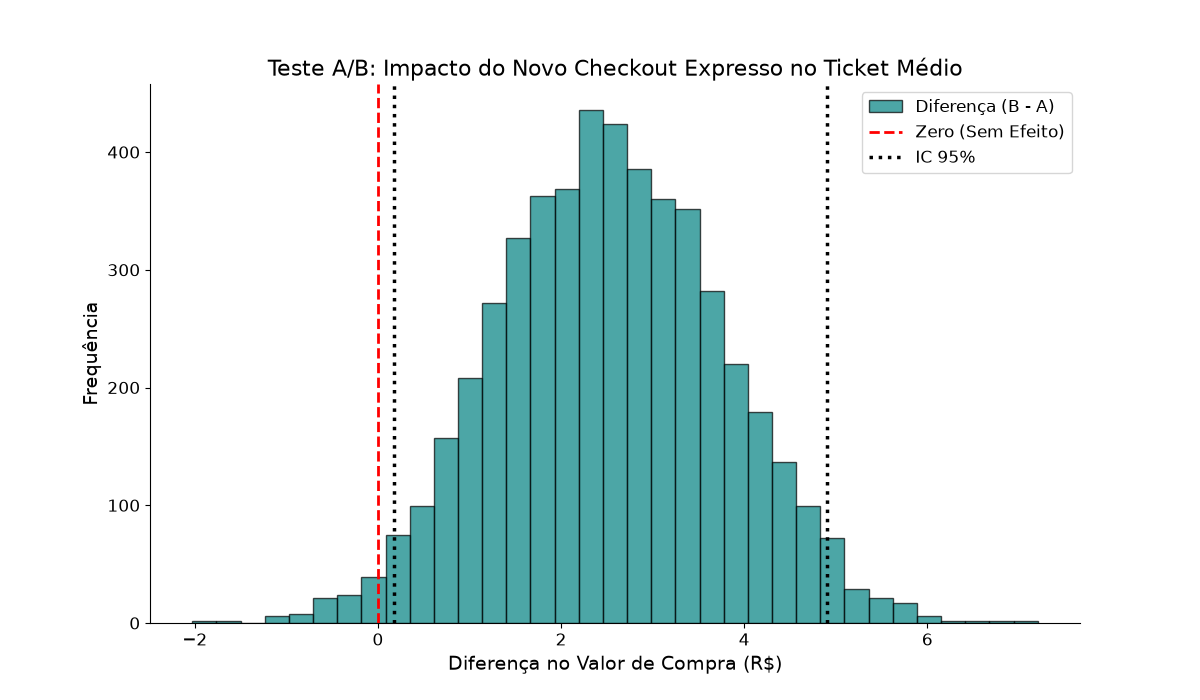
\includegraphics[width=0.85\textwidth]{04_ab_teste_ecommerce.png}
\end{frame}

\begin{frame}{Explicação: Teste A/B de Ticket Médio}
    \begin{block}{Interpretação de Negócio (Checkout Expresso)}
        \begin{itemize}
            \item \textbf{Efeito Estimado:} A diferença observada de ticket médio ($B - A$) é de $+\text{R\$} 2.53$.
            \item \textbf{Decisão Estatística:} O $IC$ (Intervalo de Confiança) de 95\% da diferença obtida via Bootstrap é $[\text{R\$} 0.18, \text{R\$} 4.90]$.
            \item \textbf{Ausência de Zero:} Como o limite inferior do $IC$ (Intervalo de Confiança) está estritamente acima de zero, o novo Layout B traz um ganho real e não puramente aleatório. Recomendamos implementar em produção.
        \end{itemize}
    \end{block}
\end{frame}

